\documentclass[../mathNotesPreamble]{subfiles}
\begin{document}
%  \relscale{1.4}
  \section{6.7: Physical Applications}

  \begin{defn*}[Mass of a One-Dimensional Object]
    Suppose a thin bar or wire is represented by the interval $a\leq x\leq b$ with a density function $\rho$ (with units of mass per length). The \textbf{mass} of the object is
      \[m=\int_a^b \rho(x)\,dx.\]
  \end{defn*}

  \begin{ex*}
    A thin bar, represented by the interval $0\leq x\leq 4$, has density in units of kg/m given by $\rho(x)=5e^{-2x}$. What is the mass of the bar?
  \end{ex*}
  \vspace*{\stretch{1}}
  \pagebreak

  \begin{defn*}[Work]
    The work done by a variable force $F$ moving an object along a line from $x=a$ to $x=b$ in the direction of the force is
      \[W=\int_a^b F(x)\,dx.\]
  \end{defn*}

  \begin{ex*}
    According to \textbf{Hooke's Law}, the force required to keep a spring in a compressed or stretched position $x$ units from the equilibrium position is $F(x)=kx$, where the positive spring constant $k$ measures the stiffness of the spring.
    \vspace*{\baselineskip}

    Suppose a force of $40$ N is required to stretch a spring $0.1$ m from its equilibrium position. Assuming the spring obeys Hooke's Law, how much work is required to stretch the spring $0.4$ m beyond is equilibrium position? 
  \end{ex*}
  \vspace*{\stretch{1}}

  \begin{ex*}[Work from force]
    How much work is required to move an object from $x=1$ to $x=3$ (measured in meters) in the presence of a force (in N) given by $F(x)=\dfrac{2}{x^2}$ acting along the $x$-axis?
  \end{ex*}
  \vspace*{\stretch{0.5}}
  \pagebreak

  \begin{ex*}
    Imagine a chain of length $L$ meters with constant density $\rho$ kg/m is hanging vertically. Using $g$ to represent the acceleration due to gravity, the work required to lift the chain is
      \[W=\int_0^L \rho g\parens{L-y}\,dy\]
    A $50$ meter long chain hangs vertically from a cylinder attached to a winch. Assume there is no friction in the system and the chain has a density of $3$\nobreakspace kg/m. How much work is required to wind the entire chain onto the cylinder if a $60$-kg load is attached to the end of the chain? Use $g$ for the acceleration due to gravity.
  \end{ex*}
  \vspace*{\stretch{1}}
  \pagebreak

  \begin{ex*}
    A $30$-meter long rope hangs freely from a ledge. The rope has a density of $5$\nobreakspace kg/m.  How much work is done if the top $1/3$ of the rope is pulled up to the ledge? Use $g$ for the acceleration due to gravity.
  \end{ex*}
  \vspace*{\stretch{1}}
  \pagebreak

  \begin{thmBox*}[Procedure: Solving Pumping Problems]
    \begin{enumerate}
      \item 
        Draw a $y$-axis in the vertical direction (parallel to gravity) and choose a convenient origin. Assume the interval $\sbrkt{a,b}$ corresponds to the vertical extent of the fluid.
      \item 
        For $a\leq y\leq b$, find the cross-sectional area $A(y)$ of the horizontal slices and the distance $D(y)$ the slices must be lifted.
      \item 
        The work required to lift the water is
          \[W=\int_a^b \rho gA(y)D(y)\,dy.\]
    \end{enumerate}
    \textit{Note}: Lifting problems are a special case of pumping problems where $A(y)=1$.
  \end{thmBox*}

  \begin{ex*}
    A water tank is shaped like an inverted cone with height 6 meters and base radius 1.5 meters. If the tank is full, how much work is required to pump the water to the level of the top of the tank and out of the tank? Use $g$ for the acceleration due to gravity and note that the density of water is $1000$ kg/m$^3$. 
  \end{ex*}
  \begin{flushright}
    \def\xx{2.75}
    \def\xxx{\xx+2.15}
    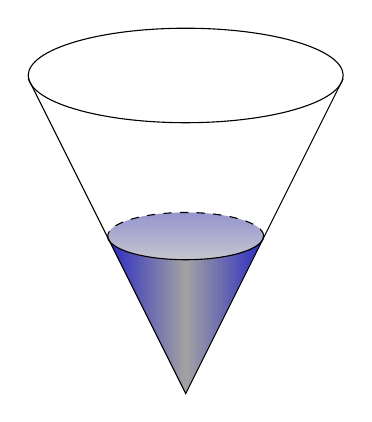
\begin{tikzpicture}
      \fill[
        top color=blue!90,
        bottom color=blue!15,
        shading=axis,
        opacity=0.25
        ] 
      (0,-2) circle (0.99cm and 0.30cm);
      \fill[
        left color=blue,
        right color=blue,
        middle color=gray!40,
        shading=axis,
        opacity=0.60
        ] 
      (1,-2) -- (0,-4) -- (-1,-2) arc (180:360:0.99cm and 0.30cm);
      \begin{scope}
        \clip (-1,-2) rectangle (2,-1cm);
        \draw[dashed] (0,-2) circle(0.99cm and 0.30cm);
      \end{scope}
      \begin{scope}
        \clip (-1,-2) rectangle (1,-3cm);
        \draw (0,-2) circle(0.99cm and 0.30cm);
      \end{scope}
      \draw (0,0.04) circle(2.0cm and 0.60cm);
      \draw (-2,0) -- (0,-4) -- (2,0);
    \end{tikzpicture}
  \end{flushright}
  \vspace*{\stretch{1}}
  \pagebreak

  \begin{ex*}(Pumping gasoline)
    A cylindrical tank with a length of $10$ m and a radius of $5$ m is on its side and half full of gasoline. How much work is required to empty the tank through an outlet pipe at the top of the tank? The density of gasoline is $\rho=737$\,kg/m$^3$
  \end{ex*}
  \begin{flushright}
    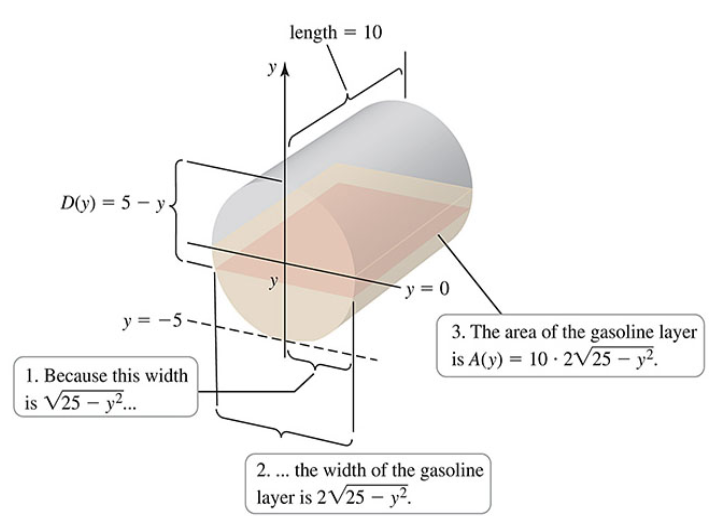
\includegraphics[width=0.45\linewidth]{../images/briggs_06_07/fig06_78}
  \end{flushright}
  \vspace*{\stretch{1}}
  \pagebreak

  \begin{thmBox*}[Procedure: Solving Force-on-Dam Problems]
    \begin{enumerate}
      \item 
        Draw a $y$-axis on the face of the dam in the vertical direction and choose a convenient origin (often taken to be the base of the dam).
      \item 
        Find the width function $w(y)$ for each value of $y$ on the face of the dam.
      \item 
        If the base of the dam is at $y=0$ and the top of the dam is at $y=a$, then the total force on the dam is
          \[F=\int_0^a \rho g\underbrace{(a-y)}_{\textnormal{depth}}\underbrace{w(y)}_{\textnormal{width}}\,dy.\]
    \end{enumerate}
  \end{thmBox*}

  \begin{ex*}
    The figure to the right shows the shape and dimensions of a small dam. Assuming the water level is at the top of the dam, find the total force on the face of the dam. Use $\rho$ for the density of the water and $g$ for the acceleration due to gravity.
  \end{ex*}
  \begin{flushright}
    \begin{tikzpicture}[scale=1.25]
      \fill[
        draw = ClemsonOrange,
        line width = 1.5pt, 
        top color=gray!30,
        middle color=ClemsonPurple!50,
        bottom color=ClemsonPurple,
        shading=axis,
        opacity=0.50
        ] 
      (-1,3) -- (0,0) -- (1,3) -- cycle;
      \draw[decorate, decoration={brace, amplitude=5pt}] (-1,3.125)--(1,3.125) node[pos=0.5, above, inner sep=7.5pt] {$20$ m};
      \draw[decorate, decoration={brace, amplitude=5pt}] (-1.125,0)--(-1.125,3) node[pos=0.5, left, inner sep=7.5pt] {$30$ m};
    \end{tikzpicture}
  \end{flushright}
  \vspace*{\stretch{1}}
  \pagebreak

  \begin{ex*}{Force on a building}
    A large building shaped like a box is $50$ m high with a face that is $80$ m wide. A strong wind blows directly at the face of the building, exerting a pressure of $150$ N/m$^2$ at the ground and increasing with height according to $P(y)=150+2y$, where $y$ is the height above the ground. Calculate the total force on the building, which is a measure of the resistance that must be included in the design of the building.
  \end{ex*}
  \vspace*{\stretch{1}}
  \pagebreak

\end{document}
